%\newif\ifpdf
%\ifx\pdfoutput\undefined
%\pdffalse % we are not running PDFLaTeX
%\else
%\pdfoutput=1 % we are running PDFLaTeX
%\pdftruep
%\fi

\documentclass[a4paper]{article}
\usepackage[swedish, english]{babel}
\usepackage[T1]{fontenc}

%\ifpdf
%\usepackage[pdftex]{graphicx}
%\renewcommand{\encodingdefault}{T1}
%\renewcommand{\rmdefault}{pad}
%\pdfcompresslevel=9
%\else
\usepackage{graphicx}
%\fi

\usepackage{url}                      % (handy if you reference a URL.)
\makeatletter
\def\url@leostyle{
  \@ifundefined{selectfont}{\def\UrlFont{\sf}}{\def\UrlFont{\small\ttfamily}}}
\makeatother
\urlstyle{leo}
\usepackage{fancyhdr}
\pagestyle{fancy}
\lhead{\small{\textit{Henrik Frisk}}}
\chead{}
\rhead{\small{\textit{The Integra Environment}}}

\usepackage{verbatim}

\title{Suggestions for the Integra Environment.}
\author{{Henrik Frisk}\\{\small Malm� Academy of Music - Lund
University}\\{\small henrik.frisk@mhm.lu.se}\\{\small http://www.henrikfrisk.com/}}
\date{\today}

\begin{document}
\selectlanguage{english}
\maketitle

\thispagestyle{empty}
\section{Introduction}

Following the presentations by Jamie Bullock, Birmingham and Henrik
Sundt, NOTAM at our meeting in Birmingham last month and the discussions
at the Integralive web site I have a suggestion for an XML file
structure that would allow for pieces developed in or transferred to the
Integra environment to be easily stored, upgraded, and transferred to
different technologies. Further, developing a graphical editor for the
XML files that would act as a hub between the synthesis engine(s), the
database and the GUI would allow for using multiple pieces of synthesis
and analysis software in the same piece of music. Finally, this document
also approaches the timeline issue.

The Integra goals as they were defined in the presentation by Henrik
Sundt and NOTAM in Birmingham have been the guideline for the
suggestions presented in this document:
\begin{itemize}
 \item User friendly tool for live electronics.
 \item Methods for preservation of works.
 \item Encourage inter-program communication, and contribute to a
       modular environment for live electronics.
\end{itemize}

Apart from the already introduced technologies (OSC and SQL of some
flavor) this suggestion also relies on:
\begin{itemize}
 \item XML (see {\url{http://www.w3schools.com/xml/xml_whatis.asp}})
 \item Jack (see {\url{http://jackit.sourceforge.net/}})
 \item SMIL (see {\url{http://www.w3schools.com/smil/smil_intro.asp}})
 \item VST and LADSPA
\end{itemize}

An overview of the structure of the connections between all the pieces
referred to in this document can be seen in figure \ref{structure}.

The assets of the suggestions in this document may be summarized as:
\begin{itemize}
 \item Completely open as to choice of synthesis/analysis engine.
 \item Different synthesis/analysis engines can easily be compared and
       exchanged.
 \item An integrated format in wich a complete description of the
       electronics in a piece of music can be saved independently of the
       technology used to implement it.
 \item Each file can be validated generally and specifically against an
       external Integra DTD (Document Type Definition).
\end{itemize}

The drawbacks may be summarized as:
\begin{itemize}
 \item Uses several standards.
 \item Possibly requires a larger programming effort from the Integra
       team.
 \item Jack does not work on Windows (yet).
\end{itemize}

\begin{figure}[!h]
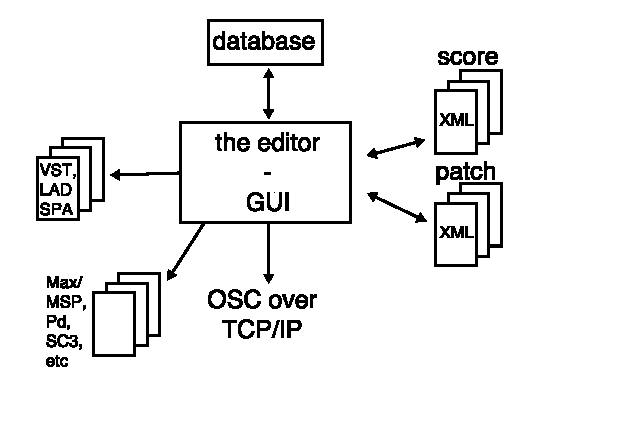
\includegraphics[width=0.9\textwidth]{./structure}
\caption{Structure.} \label{structure}
\end{figure}

\section{File structure for storing Integra 'patches'.}

Following is a very generalized example of how the Integra xml file
format could look like. This particular example describes the single
oscilliator 'patch' in figure \ref{graph}:

{\small \verbatiminput{example.xml} }

\begin{figure}[!hbt]
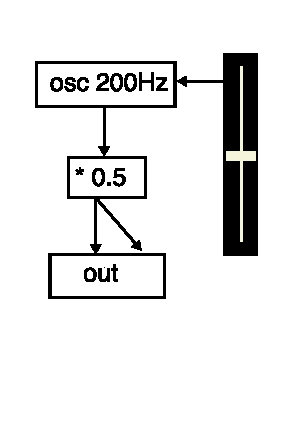
\includegraphics[width=0.4\textwidth]{./simpleSynth}
\caption{Simple patch example.} \label{graph}
\end{figure}

The file has a {\small \texttt{<head>}} tag and a {\small
\texttt{<body>}} tag. The head tag would hold information on the number of
physical and virtual audio inputs and outputs etc. The body
tag contains the actual modules and their attributes.

The XML structure follows the OSC class hierarchy for each module
contained in it and for each module it holds the attributes for default
values, control sources, information on mapping of values etc.

\section{The editor}

The file above can be generated in the editor simply by adding and
connecting objects in a Max-Pd fashion. However, \emph{only objects of
the abstract base class} can be added in the GUI. In the example above
the only two objects that are added are one object of class {\small
\texttt{Integra/GeneralAudioModule/GeneralSynth}} and one of class
{\small \texttt{Integra/General\-Controller/GeneralFader}} (the gain
module would be implied at any sound generating or processing
output\footnote[1]{Exactly how, and what modules should be combined to
accomplish a functional meta-module such as a synthesizer is an issue
that, no matter how the final design will look like, needs to be
discussed in greater detail.}). After the abstract class of the object
has been chosen and is displayed an instance of this class can be
created. The list of available modules is dynamically fetched from the
database and in the case of a {\small \texttt{GeneralSynth}} it could
for example be:
\begin{itemize}
 \item FM
       \begin{itemize}
	\item Pd
	      \begin{itemize}
	       \item hexter
	       \item dssi
	      \end{itemize}
	\item MIDI
	      \begin{itemize}
	       \item DX7
	      \end{itemize}
       \end{itemize}
 \item Additative
       \begin{itemize}
	\item ...
       \end{itemize}
 \item JAMOMA
\end{itemize}

For the chosen module the documentation is included in the XML file
directly. Using XLS transforms this allows for exporting the
documentation to any one of a number of formats (PDF, HTML, etc) as well
as displayed within the editor.  The 'patch building GUI' would obviously
be significantly simpler to learn, understand and implement than that of
Max or Pd. 

After the Integra XML file is loaded or created a set of on screen
faders (or whatever graphical component is the most suitable for the
particular parameter) corresponding to the objects created are
automatically generated.

\section{The processing.}

Once the structure of the synthesis/processing/analysis patch is created
it needs to be exported to the actual software packages handling the
audio processing. One way this could be done is to support a plug-in
structure in which support for a specific piece of software can be
implemented. With such plug-ins, or parsers, the Integra XML file would
be used to render a fully functional and Integra OSC namespace
compatible patch in the desired program, be it PD, Max/MSP,
SuperCollider or any combination of software.

The other way to work would be to use modules from different software
packages, i.e. using Max/MSP and Jitter for realtime analysis of video
input, using that data to control the synthesis implemented in
SuperCollider and playing back samples on a hardware sampler. By using
Jack as the audio server audio streams can be sent between applications
with low latency. Presumably a fully functional and Integra OSC
compliant module should be contained in the database and easily
downloaded to the client. With a class structure of OSC-to-MIDI
transformation modules hardware systems could easily be integrated into
such a system. Even without the use of Jack this model is possible with
external mixing - there is no need for all the modules to reside on the
same computer.

\section{The timeline}

The issue of a timeline - basically the possibility to automate control
signals and to trigger chains of events at certain points in time - was
discussed at our meeting in Birmingham. In this suggestion I argue that
we should separate the time critical information, the cue list, from the
'patch' mainly for clarity.

Some aspects to consider:
\begin{itemize}
 \item How is the cue list edited?
 \item How is the state of all modules updated when rehearsing?
 \item How are triggers handled? Tempo changes?
\end{itemize}

One suggestion that effortlessly would deal with all of the above and at
the same time liberate us from having to implement our own timeline
editor would be to let the editor described above export a light-weight
VST or LADSPA plug-in that holds all the parameters contained in the
Integra XML file. The only thing the plug-in does is transformation of
VST/LADSPA control signals to OSC. Loading the plug-in in a sequencer of
choice allows the user to edit all the parameters using all the tools
available in the sequencer and at the same time sending the relevant
data to the 'patches'. A special cue plug-in could be used to handle cue
points in the 'score'. Once the editing is done, the entire cue list is
exported to an Integra score file-format which can be loaded in the
editor. Once it is loaded in the editor the score playback is controlled
by play, stop, pause and step buttons in the GUI of the editor. The
option of patching in a user input module (sensor, foot pedal, etc.)
should also be present.

\subsection{Assets}
\begin{itemize}
 \item For those used to working in a sequencer, the environment is well
       known.
 \item Preparing a cue list for a work in which the instrumental part is
       already recorded becomes very convenient - load the track into
       the sequencer and load the plug-ins and draw the automation.
 \item Relieves the Integra team of having to develop their own
       timeline.
 \item Since exporting the data would write every value at some control
       rate (rather than the ususal line segments) allows for complete
       parameter update at every point along the timeline.
 \item Making use of existing technology.
\end{itemize}

\subsection{Drawbacks}
\begin{itemize}
 \item Relies on external protocols (VST, LADSPA) and technology
       (sequencer). 
 \item The sequencer timeline may not be the most appropriate
       representation for recording data in some styles of music.
 \item The extra steps of exporting of a plug-in, loading it in a
       sequencer etc. is not very intuitive.
\end{itemize}

\subsection{The score file format}
An XML format for synchronizing streaming media, SMIL (see
{\url{http://www.w3schools.com/smil/smil_intro.asp}}) already exists and
is now at version 2.0. It is my belief that a lot would be gained by
using the SMIL format as a starting point and use our own
namespace that extends the basic functionality of SMIL. A simple SMIL
file that plays back a soundfile from a server once and then exits can
be seen below. This particular file uses the Real Networks (RealAudio)
namespace extensions. 

{\small \verbatiminput{example.smil} }

An advantage with using the SMIL format is that images and video may
easily be incorporated and synchronized with the audio for artistic as
well as documentation purposes.

\section{Conclusion}

I have discussed the issues brought up in this document with my
collegues in Malm�, and to some extent with Henrik Sundt after the
Birmingham meeting. This document should be regarded as a rough sketch
and I have quite possibly overlooked some things. However, if the ideas,
or some of the ideas, put forward in this document appear to be
interesting to the rest of the Scientific Group, a more detailed and
well structured presentation could be given at our meeting in Krakow in
May.

Using XML for storing the structure of the patches and the control data
needed to 'play' a piece of music containing elements of live
electronics has many advantages, but especially the possibility for
including documentation in the files combined with publicly available
tools for transforming this data to any number of output formats makes
it an attractive possibility for the Integra project.


\end{document}